\documentclass[10pt,letterpaper,spanish,twoside]{report}

\usepackage{practica}
\usepackage{graphicx}
\usepackage{float}
\DeclareGraphicsExtensions{.bmp,.png,.pdf,.jpg}
\newcommand{\docdate}{
  \vspace{2em}
   \begin{flushright}
     Ciudad de México. \datedayname~\today.
   \end{flushright}
  \vspace{2em}
}

\begin{document}
\docdate

\begin{center}
 \textsc{\asignatura}\vspace{.2em}
\end{center}

\textsc{Manual del profesor}

\textsc{Práctica 0. Diseño de sistema mínimo para simular adquisición de señales bioeléctricas en tiempo real}

\textsc{Objetivo:} Construir un sistema preamplificador cuya entrada sea la señal de audio analógica generada por un dispositivo electrónico, por ejemplo: computadora, teléfono móvil, tablet, etc., dicho dispositivo reproducirá una pista de audio en formato .wav, la cual contiene información de una señal de origen fisiológico, en otras palabras, se estará simulando la adquisición de señal de paciente en tiempo real.

Se sugiere utilizar el amplificador de instrumentación INA114AP
\newline El archivo de la hoja de especificaciones es INAW14AP.PDF

\textsc{Actividades}
\begin{enumerate}
 \item Para lograr una amplificación entre $\pm$ 1.5 V y $\pm$ 5.5 V. utilizar un potenciometro de presición de 50K$\Omega$, este valor fue elegido debido a que se requiere una ganancia de 100 ya que las señales fisiológicas se encuentran en el orden de mV.
 \item Conectar el circuito como se observa en la figura~\ref{contexto:INA114}
 \begin{figure}[H]
 	\centering
 	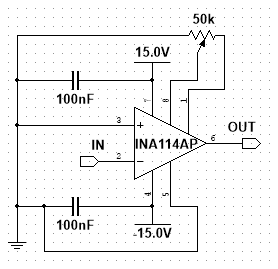
\includegraphics[scale=0.7]{INA114.PNG}
 	\caption{Conexiones del amplificador de instrumentación}
	\label{contexto:INA114}
 \end{figure}
 \item A continuación se observa en la figura 2 la respuesta en frecuencia del amplifcador con 15 mediciones por decada y 10 alrededor de la frecuencia de corte. Para observar el código para la caracterización consultar el archivo INA114AP.ipynb.
 \newline De acuerdo con los datos proporcionados en la hoja de especificaciones del amplificador, se comprueba que al tener una ganancia de 100, el sistema funciona de manera lineal hasta 10KHz
 \begin{figure}[H]
 	\centering
 	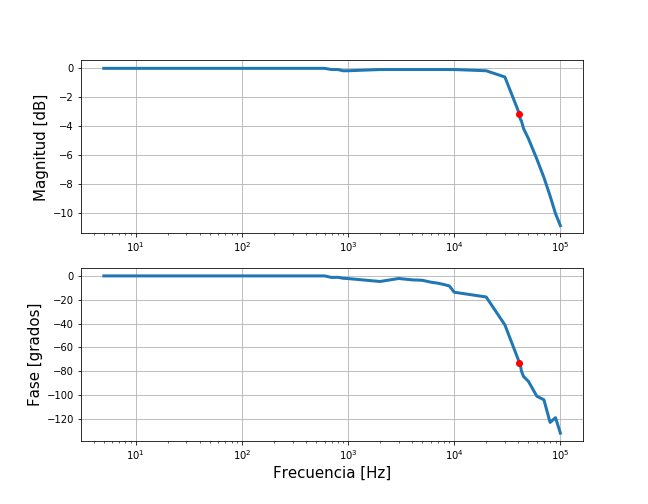
\includegraphics[scale=0.5]{RF_AI.PNG}
 	\caption{Respuesta en frecuencia}
	\label{contexto:figura}
 \end{figure}
 \item Evaluar el funcionamiento del simulador de paciente con señales de origen biomédico, las cuales fueron descargadas del banco de señales de physionet, el procesamiento de dichas señales se puede consultar en el archivo Señales$\_$utilizadas.ipynb 
 \newline En las siguiente figuras se puede observar que el amplificador funciona correctamente.\\AGREGAR FIGURAS DE OSCILOSCOPIO	
\end{enumerate}


%\textsc{Nota}
%\vspace{2em}
\vfill
\begin{flushright}
\textsc{Elaboró:\\
Ma. del Rosario Aguilar Cruz\\
Enrique Mena Camilo}
\end{flushright}

\end{document}